\section{Sub-Gaussian Projections}


\begin{frame}{Matrix sketching}

\begin{center}
  
  \begin{tikzpicture}[scale=1.0]
    \draw[fill=blue!20] (-4.5,3) rectangle (-0.5,4);
%        \draw (-1.5,2.5) node {$\S$};
%        \draw (0,2.5) node {$\times$};
    \draw[fill=blue!20] (0.5,0) rectangle (3,4);
    \draw[fill=blue!20] (4,3) rectangle (6.5,4);
    \draw (1.3,2.5) node {$\S \qquad\qquad\qquad\qquad \A \qquad\qquad\qquad\tilde\A$};
%        \draw (3.5,2.5) node{$=$};
    \draw (1,3.5) node {\mbox{
        sub-gaussian\qquad$\times$\qquad data \qquad$=$\qquad sketch}};
%        \draw (5,2.5) node {$\tilde\A$};
% \draw[fill=blue!20] (1,0) rectangle (2.5,4);
%    \draw (2,2) node {\mbox{$\A$}};
%    \draw (6.5,2) node {\mbox{$\in\R^{m\times n}$}};
  \end{tikzpicture}
\end{center}
Least squares, stochastic optimization, data compression,
approximate SVD
\end{frame}
    

\begin{frame}{Residual projection matrix}

\begin{center}      
    \begin{tikzpicture}[scale=1.0]

    \draw (-3.2,-3.2) -- (3.2,3.2);
    \tkzDefPoint(0,1){A};         \tkzDefPoint(0.5,.5){A1}; \tkzDrawSegment[thick,red](A,A1);
    \tkzDefPoint(1.8,.5){B};     \tkzDefPoint(1.15,1.15){B1}; \tkzDrawSegment[thick,red](B,B1);
    \tkzDefPoint(2.5,1.5){C};   \tkzDefPoint(2,2){C1}; \tkzDrawSegment[thick,red](C,C1);
    \tkzDefPoint(-1.5,-.3){D}; \tkzDefPoint(-.9,-.9){D1}; \tkzDrawSegment[thick,red](D,D1);
    \tkzDefPoint(-2,-.3){E};    \tkzDefPoint(-1.15,-1.15){E1}; \tkzDrawSegment[thick,red](E,E1);
    \tkzDefPoint(1,1.5){F};  \tkzDefPoint(1.25,1.25){F1}; \tkzDrawSegment[thick,red](F,F1);
    \tkzDefPoint(.5,-.5){G};  \tkzDefPoint(0,0){G1}; \tkzDrawSegment[thick,red](G,G1);
    \tkzDefPoint(2,4.4/1.65){H};  \tkzDefPoint((2+4.4/1.65)/2,(2+4.4/1.65)/2){H1}; \tkzDrawSegment[thick,red](H,H1);
    \tkzDefPoint(-1,0){I};  \tkzDefPoint(-.5,-.5){I1}; \tkzDrawSegment[thick,red](I,I1);
    \tkzDefPoint(1.1,2.5){J};  \tkzDefPoint(1.8,1.8){J1}; \tkzDrawSegment[thick,red](J,J1);
    \tkzDefPoint(-1.32,-1.76){K};  \tkzDefPoint(-1.54,-1.54){K1}; \tkzDrawSegment[thick,red](K,K1);
    \tkzDefPoint(-1.5,-2.5){L};  \tkzDefPoint(-2,-2){L1}; \tkzDrawSegment[thick,red](L,L1);


    \foreach \n in {A,B,C,D,E,F,G,H,I,J,K,L} \node at (\n)[circle,fill=blue,inner
    sep=1.5pt]{};
    \foreach \n in {A1,B1,C1,D1,E1,F1,G1,H1,I1,J1,K1,L1} \node at (\n)[circle,fill=black,inner
    sep=1pt]{};        

  \end{tikzpicture}   
  \begin{align*}
    \P_{\!\perp} = \I-\tilde\A^\dagger\tilde\A\quad\text{- measures
    sketching error}
    \end{align*}
  \end{center}
\end{frame}


\begin{frame}{Main result: Expected residual projection}
    \vspace{5mm}
    
    Residual projection: $\P_{\!\perp} := \I - \P = \I -
    (\S\A)^\dagger\S\A$.

\textbf{Theorem.}  If $\S$ has i.i.d.~sub-gaussian entries:
\begin{align*}
% (1-\epsilon)\,(\gamma\A^\top\A + \I)^{-1}\preceq  \E[\P_{\!\perp}]\preceq(1+\epsilon)\, (\gamma\A^\top\A + \I)^{-1}
    \E[\P_{\!\perp}]\
   &\overset\epsilon\simeq \ (\gamma\A^\top\A + \I)^{-1}
\end{align*}
with $\gamma$ defined implicitly by
$\tr (\gamma\A^\top\A + \I)^{-1}=\tr\P_{\!\perp}$, and:
\begin{align*}
  \epsilon = O\Big(\frac1{\sqrt{\text{\footnotesize stable rank of $\A$}}}\Big).
\end{align*}

\textit{Proof.}  Random Matrix Theory!

\end{frame}

\begin{frame}{Application: Low-rank approximation}
  Error analysis for:
   \begin{enumerate}
     \item Low-rank approximation \parencite{tropp2011structure}
     \item Generalized Nystr\"om method \parencite{revisiting-nystrom}
    \end{enumerate}
    
    
    Low-rank approximation error:
    \begin{align*}
      \E[\|\A - \A\P\|_F^2]= \tr\,\A^\top\A\,\Blue{\E[\P_{\!\perp}]}
    \end{align*}
\end{frame}

\begin{frame}{Application: Optimization}
    Convergence analysis for:
  \begin{enumerate}
  \item Generalized Kaczmarz method \parencite{generalized-kaczmarz}
  \item Randomized Subspace Newton  \parencite{Gower2019}
  \item Jacobian Sketching \parencite{jacsketch}
  \end{enumerate}

    Let $\x^*$
    be the unique solution of $\A\x^*=\b$ and consider
  the iterative algorithm:
  \begin{align*}
    \x^{t+1} = \argmin_{\x} \|\x-\x^t\|^2\quad\textnormal{subject to}\quad\S\A\x=\S\b.
  \end{align*}
Then, we have:
  \begin{align*}
    \E\big[\x^{t+1}-\x^*\big] =
    \Blue{\E[\P_{\!\perp}]}\,\E\big[\x^t-\x^*\big]
  \end{align*}
\end{frame}

\begin{frame}{Application: Bias of interpolating models}
Implicit bias of interpolating models \parencite{surrogate-design}


\begin{align*}
  \underbrace{\E\Big[\argmin_{\x} \|\x\|^2\ \ \textnormal{s.t.}\ \
    \S\A\x=\S\b\Big] - \x^*}_{\text{Bias of sketched minimum norm
  solution}}
  = \Blue{\E[\P_{\!\perp}]}\,\x^*.
\end{align*}
\end{frame}

\begin{frame}{Explicit expressions for low-rank approximation error}
  Let $\sigma_i$ be the singular values of $\A$. Then:
  \begin{align*}
    \underbrace{\E\big[\|\A-\A\P\|_F^2\big]}_{\text{Error}} \ \overset\epsilon\simeq\ 
    k/\gamma
\quad \text{for \ $\gamma$ \ s.t. \ } \sum_{i}\frac{\gamma\sigma_i^2}{\gamma\sigma_i^2+1} = k.
  \end{align*}
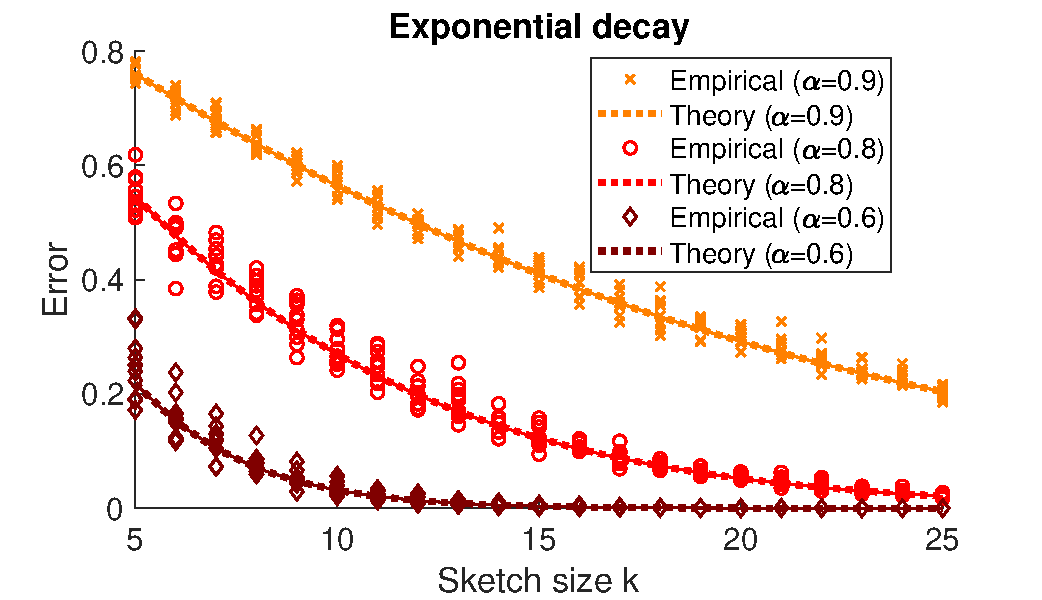
\includegraphics[width=.495\textwidth]{Figures/projections/explicit_exp}~%
\nolinebreak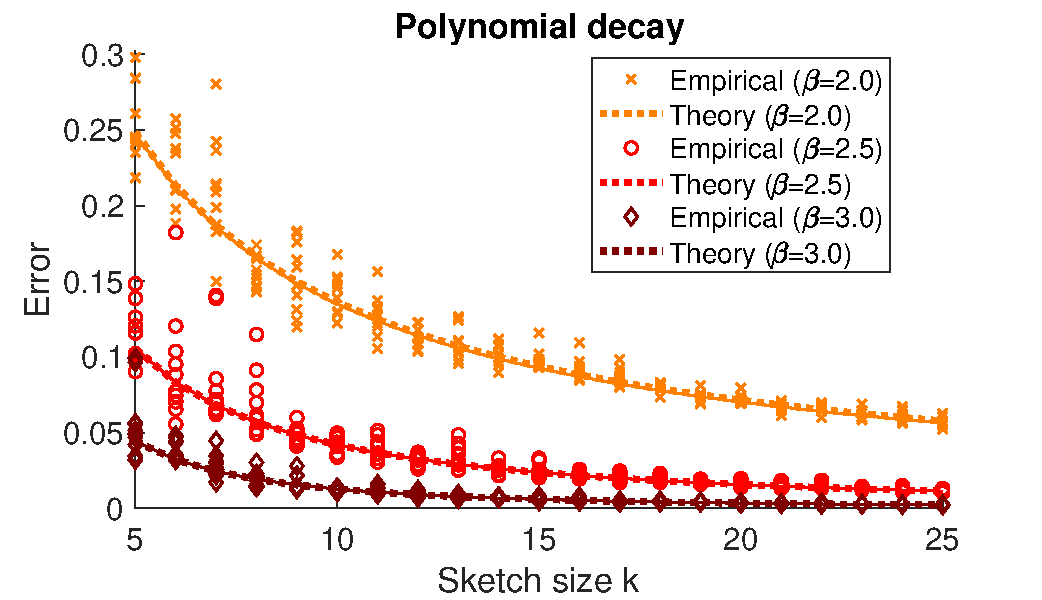
\includegraphics[width=.495\textwidth]{Figures/projections/explicit_poly}
      \begin{align*}
        \sigma_i^2&=C\cdot\alpha^{i-1}
&&&&&      \sigma_i^2
        &=C\cdot i^{-\beta}
        \\
        \text{Error} & \approx
\frac C{\sqrt\alpha}\cdot
  \frac{k}{\alpha^{-k}-1}
&&&&&  
\text{Error}&\approx
\frac{C\,k}{(k+\frac12)^\beta}\bigg(\frac{\pi/\beta}{\sin(\pi/\beta)}\bigg)^\beta
      \end{align*}
\end{frame}

\begin{frame}{Experiments on real-world datasets}
  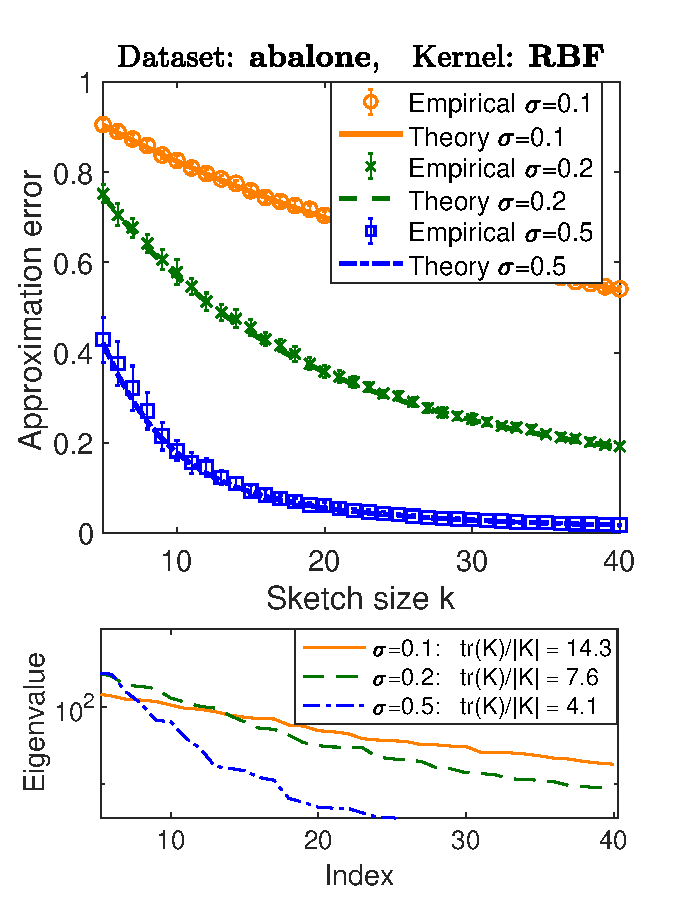
\includegraphics[width=.495\textwidth]{Figures/projections/abalone-nystrom}~%
  \nobreak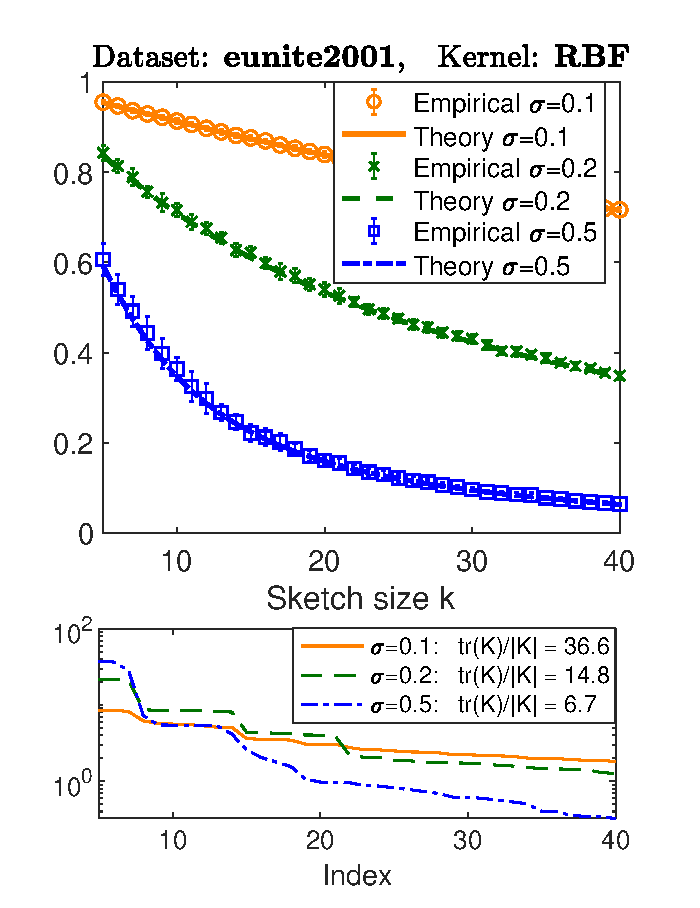
\includegraphics[width=.495\textwidth]{Figures/projections/eunite-nystrom}
\end{frame}
